\section{Result}
We have tested our method on a corpus provided by teacher. For detailed
escription of the corpus, please see former report.

\subsection{Effect On Number Of Mixtures}
We examined our GMM compared to GMM from scikit-learn.
Test is conducted on 30-speaker corpus, 30 seconds training utterance
and and 5 seconds test utterance for each speaker.

\begin{figure}[!ht]
	\centering
	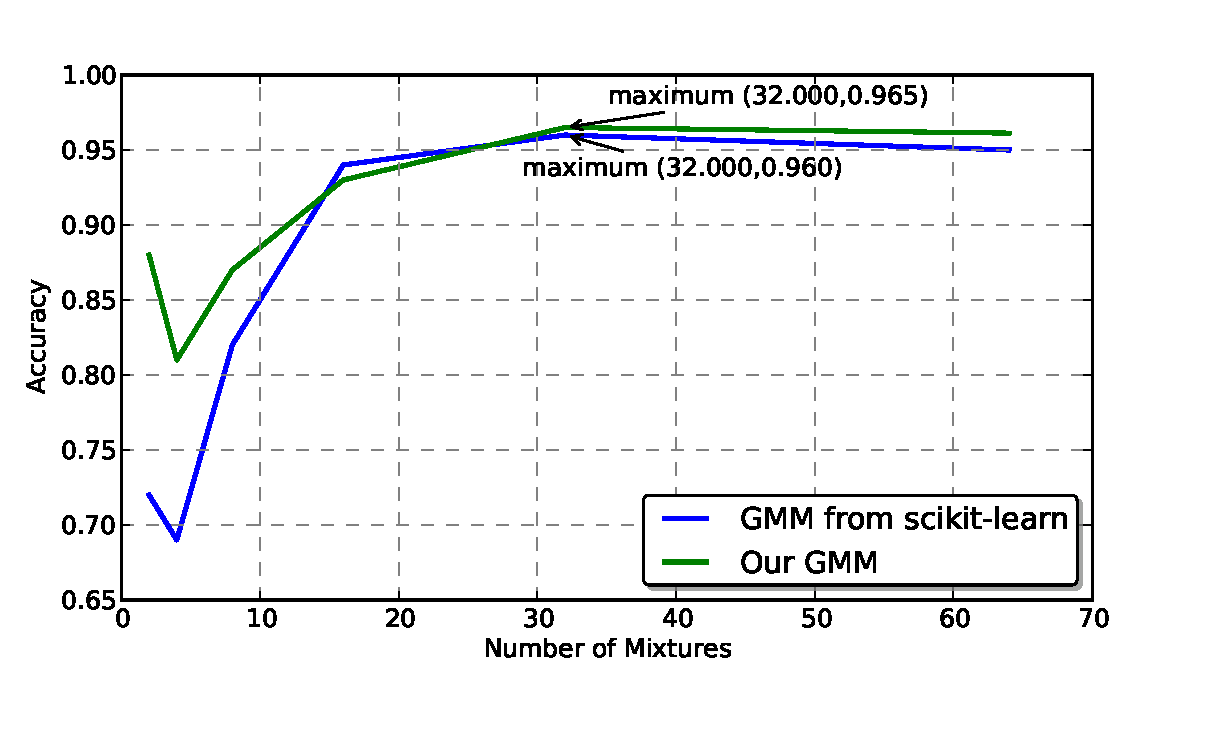
\includegraphics[width=\linewidth]{res/mixture-both.pdf}
	\caption{Accuracy curve on different number of mixtures}
\end{figure}

As the figure clearly illustrates, when number of mixtures is small,
our GMM outperforms scikit-learn version $10\%$, which indicates our
GMM models the distribution more accurate. The maximum accuracy
is when the number of mixtures is around 32, reaching $0.965$. As
the number of mixtures increase, the decrease in accuracy
may due to the overfitting to the training data.

\subsection{Effect On Number Of Speakers Enrolled}

